\subsection{Opgaver}

\begin{enumerate}
	\item Omregn følgende fra grader til radianer
	\begin{align*}
	90^\circ,&& 15^\circ,&&150^\circ,&& 45^\circ.
	\end{align*}
	
	\item Omregn følgende radianer til grader
	\begin{align*}
	\frac{\pi}{3},&&\frac{7\pi}{4},&& \frac{5\pi}{12}.
	\end{align*}
	

	
		\item Brug \href{https://www.geogebra.org/m/e2vTM4Ut}{GeoGebra} til at undersøge de trigonometriske funktioner sinus og cosinus. Bemærk at GeoGebra laver nogle afrundinger der kræver at man bruger sund fornuft når man aflæser funktionerne.
	\begin{enumerate}
		\item Bestem $\sin(0)$ og $\cos(0)$.
		\item Bestem $\sin(\frac{\pi}{2})$ og $ \cos(\frac{\pi}{2}) $.
		\item Bestem $\sin(\pi)$ og $\cos(\pi)$.
		\item Bestem $\sin(\frac{3\pi}{2}) $ og $\cos(\frac{3\pi}{2})$.
		\item Bestem $\sin(2\pi)$ og $ \cos(2\pi) $.
	\end{enumerate}
	
	 \item Udregn følgende tal
	\begin{align*}
	\sin(\frac{5\pi}{4})+\cos(\frac{\pi}{4}),&& \tan(\frac{\pi}{6})+\cos(\frac{\pi}{3}),&& \frac{\sin(\frac{\pi}{6})+\cos(\frac{\pi}{3})}{\sin(\frac{4\pi}{6})}.
	\end{align*}
	
	\begin{figure}
		\centering
		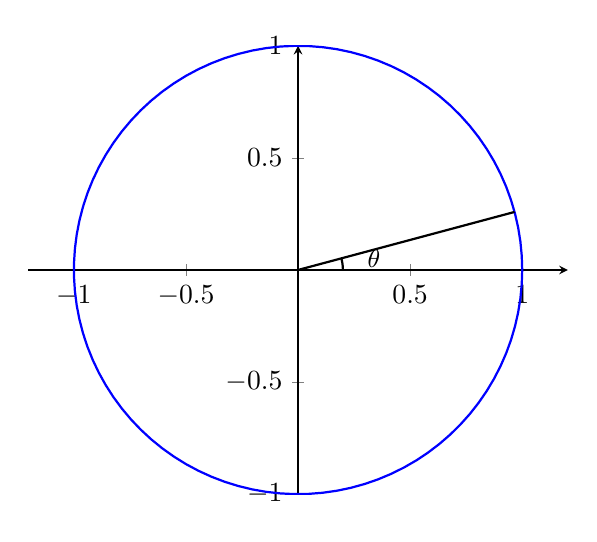
\begin{tikzpicture}
		\begin{axis}[xmin=-1,xmax=1,ymin=-1,ymax=1,axis x line=center,
		axis y line=center, axis equal]
		\addplot[blue,domain=0:2*pi,thick, samples=100] ({cos(deg(x))},{sin(deg(x))});
		\addplot[domain=0:(sqrt(6)+sqrt(2))/4,thick] {(2-sqrt(3))*x};
		\addplot[domain=0:pi/12,thick,samples=100] ({0.2*cos(deg(x))},{0.2*sin(deg(x))}) node[label={[label distance=2pt]0.5:\small$\theta$},pos=1] {};
		\end{axis}
		\end{tikzpicture}
		\caption{Opgave~\ref{it:trig1}}
		\label{fig:trig1}
	\end{figure}
	

	\item Brug sumformlerne til at vise formlerne $\sin(-\theta)=-\sin(\theta) $ og $\cos(-\theta)=\cos(\theta) $. Se evt. \href{https://www.geogebra.org/m/e2vTM4Ut}{GeoGebra}. (Hint $\cos(-\theta)=\cos(0-\theta)$ og $\sin(-\theta)=\sin(0-\theta)$).
	
	\item Brug \href{https://www.geogebra.org/m/e2vTM4Ut}{GeoGebra} til at formode en sammenhæng mellem $\cos(\theta-\frac{\pi}{2})$ og $\sin(\theta)$. Brug efterfølgende sumformlerne til at be- eller afkræfte formodningen.
	  
	  	\item \label{it:trig1} I Figur~\ref{fig:trig1} er en vinkel på $\theta$ indtegnet i enhedscirklen. Skitser vinklerne
	  \begin{align*}
	  \theta+ \frac{\pi}{2},&& \pi-\theta,&& \theta +3\pi,&& \frac{7\pi}{4}-\theta.
	  \end{align*}
	  
	
	 
	 \item Bestem to forskellige løsninger til ligningerne 
	 \begin{align*}
	 \sin(x)=\frac{\sqrt{3}}{2},&& \cos(x-\pi)=-\frac{\sqrt{2}}{2},&& 2\sin^2(x)+5\sin(x)+2=0.
	 \end{align*}

	\item Brug enhedscirklen til at vise idiotformlen
	\begin{align*}
	\sin^2x+\cos^2x=1.
	\end{align*}
	(Hint: Pythagoras.)

	\item Udregn følgende
	\begin{align*}
	\cos(-\frac{3\pi}{4}),&& \sin(\frac{5\pi}{6}),&&\tan(\frac{5\pi}{4}),&& \cos(\frac{5\pi}{3}).
	\end{align*}
	
	\item\label{it:trig2} Vis at $\sin(2\theta)=2\cos(\theta)\sin(\theta)$. (Hint: Brug sumformlerne)

	\item Løs ligningen $16\sin^2(x)\cos^2(x)=3$ for $x\in [0,\pi]$. (Hint: Brug formlen fra Opgave~\ref{it:trig2})
	
	\item Udregn
	\begin{align*}
	\cos(\frac{15\pi}{4}),&& \tan(\frac{14\pi}{6}),&& \sin(-\frac{10\pi}{3}),&& \tan(\frac{10 \pi}{5}).
	\end{align*}
	
	\item Vis at $\tan(x+\pi)=\tan(x)$ for alle hvor tangens er defineret. (Hint: Brug sumformlerne.)
	
	\item Løs ligningen $\sin^2(\theta)+3\cos^2(\theta) =2$ for $\theta\in [0,\frac{\pi}{2}]$.(Hint: Idiotformlen)
	
	\item \label{it:trig3} I denne opgave beviser vi nogle af de eksakte værdier for sinus og cosinus til vinklerne $ \frac{\pi}{6}$ og $ \frac{\pi}{6} $.
	
	\begin{enumerate}
		\item Vis at $\sin(\frac{\pi}{6})=\frac{1}{2}$ ved at regne på trekanten i Figur~\ref{fig:trig3}. (Hint: Hvad kan man sige om sidelængderne i trekanten?)
		
		\item Brug idiotformlen til at vise at $\cos(\frac{\pi}{6})=\frac{\sqrt{3}}{2}$.
		
		\item Vis at $\sin(\frac{\pi}{3})=\frac{\sqrt{3}}{2}$. (Hint: $ \sin(\frac{\pi}{3})=\sin(\frac{\pi}{6}+\frac{\pi}{6}) $)
		
		\item Brug idiotformlen til at vise at $\cos(\frac{\pi}{3})=\frac{1}{2}$.
		
	\end{enumerate}
		
	\begin{figure}
		\centering
		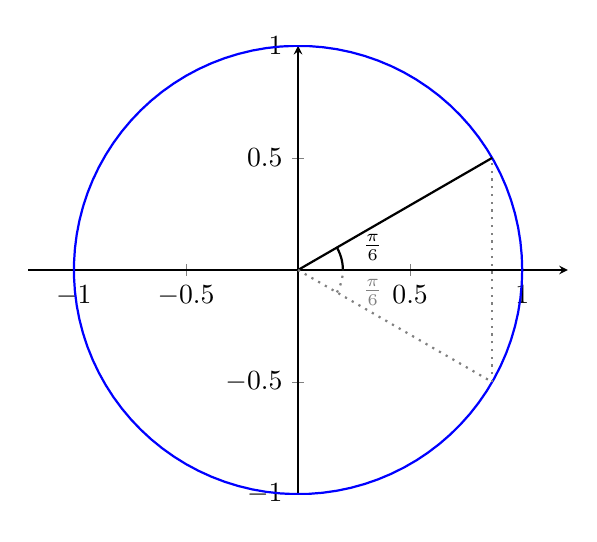
\begin{tikzpicture}
		\begin{axis}[xmin=-1,xmax=1,ymin=-1,ymax=1,axis x line=center,
		axis y line=center, axis equal]
		\addplot[blue,domain=0:2*pi,thick, samples=100] ({cos(deg(x))},{sin(deg(x))});
		\addplot[domain=0:sqrt(3)/2,thick] {1/sqrt(3)*x};
		\addplot[domain=0:pi/6,thick,samples=100] ({0.2*cos(deg(x))},{0.2*sin(deg(x))}) node[label={[label distance=2pt]0.5:\small$\frac{\pi}{6}$},pos=1] {};
		\addplot[domain=0:sqrt(3)/2,thick,gray,dotted] {-1/sqrt(3)*x};
		\addplot[domain=-pi/6:0,thick,samples=100,gray,dotted] ({0.2*cos(deg(x))},{0.2*sin(deg(x))}) node[label={[label distance=2pt]0.5:\small$\frac{\pi}{6}$},pos=0] {};
		\addplot[dotted,gray,thick] coordinates {(sqrt(3)/2, -1/2) (sqrt(3)/2, 1/2)};
		\end{axis}
		\end{tikzpicture}
		\caption{Opgave~\ref{it:trig3}}
		\label{fig:trig3}
	\end{figure}

		\item \label{it:trig4} I denne opgave beviser vi nogle af de eksakte værdier for sinus og cosinus til vinklerne $ \frac{\pi}{4}$.
		\begin{enumerate}
			\item Vis at $\sin(\frac{\pi}{4})=\frac{\sqrt{2}}{2}$ ved at regne på trekanten i Figur~\ref{fig:trig4}.(Hint: Pythagoras) 
			\item Brug idiotformlen til at vise at $\cos(\frac{\pi}{4})=\frac{\sqrt{2}}{2}$. 
		\end{enumerate}
	
	\begin{figure}
		\centering
		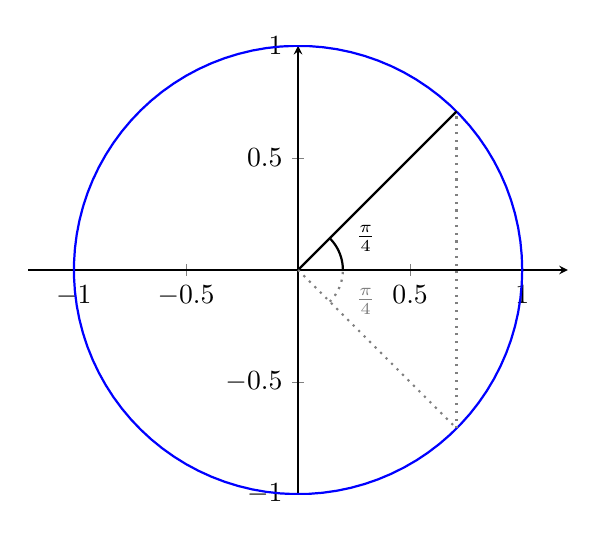
\begin{tikzpicture}
		\begin{axis}[xmin=-1,xmax=1,ymin=-1,ymax=1,axis x line=center,
		axis y line=center, axis equal]
		\addplot[blue,domain=0:2*pi,thick, samples=100] ({cos(deg(x))},{sin(deg(x))});
		\addplot[domain=0:sqrt(2)/2,thick] {1*x};
		\addplot[domain=0:pi/4,thick,samples=100] ({0.2*cos(deg(x))},{0.2*sin(deg(x))}) node[label={[label distance=2pt]0.5:\small$\frac{\pi}{4}$},pos=1] {};
		\addplot[domain=0:sqrt(2)/2,thick,gray,dotted] {-1*x};
		\addplot[domain=-pi/4:0,thick,samples=100,gray,dotted] ({0.2*cos(deg(x))},{0.2*sin(deg(x))}) node[label={[label distance=2pt]0.5:\small$\frac{\pi}{4}$},pos=0] {};
		\addplot[dotted,gray,thick] coordinates {({sqrt(2)/2}, -{sqrt(2)/2}) ({sqrt(2)/2}, {sqrt(2)/2})};
		\end{axis}
		\end{tikzpicture}
		\caption{Opgave~\ref{it:trig4}}
		\label{fig:trig4}
	\end{figure}

	\item \label{it:trig5}I denne opgave beviser vi nogle af de eksakte værdier for sinus og cosinus til vinklerne $ \frac{\pi}{12}$ og $ \frac{5\pi}{12} $.
	\begin{enumerate}
%		\item Brug Figur~\ref{fig:trig5} at $\sin(\frac{\pi}{12})=\frac{\sqrt{2-\sqrt{3}}}{2}$. (Hint: Brug cosinusrelationen)
%		\item Brug idiotformlen til at bestemme $\cos(\frac{\pi}{12})$. 
		\item Bestem $\cos(\frac{\pi}{12})$ og $\sin(\frac{\pi}{12})$ ved at bruge sumformlerne. (Hint: $ \frac{\pi}{12}=\frac{\pi}{3}-\frac{\pi}{4} $)
		\item  Bestem $\cos(\frac{5\pi}{12})$ og $\sin(\frac{5\pi}{12})$ ved at bruge sumformlerne. (Hint: $ \frac{5\pi}{12}=\frac{\pi}{6}+\frac{\pi}{4} $)
	\end{enumerate}
	
	
%	\begin{figure}
%		\centering
%		\begin{tikzpicture}
%		\begin{axis}[xmin=-1,xmax=1,ymin=-1,ymax=1,axis x line=center,
%		axis y line=center, axis equal]
%		\addplot[blue,domain=0:2*pi,thick, samples=100] ({cos(deg(x))},{sin(deg(x))});
%		\addplot[domain=0:(sqrt(6)+sqrt(2))/4,thick] {(2-sqrt(3))*x};
%		\addplot[domain=0:pi/12,thick,samples=100] ({0.2*cos(deg(x))},{0.2*sin(deg(x))}) node[label={[label distance=2pt]0.5:\tiny$\frac{\pi}{12}$},pos=1] {};
%
%		\addplot[domain=0:(sqrt(6)+sqrt(2))/4,thick,gray,dotted] {-(2-sqrt(3))*x};
%		\addplot[domain=-pi/12:0,thick,samples=100,gray,dotted] ({0.2*cos(deg(x))},{0.2*sin(deg(x))}) node[label={[label distance=2pt]0.5:\tiny$\frac{\pi}{12}$},pos=0] {};
%		\addplot[dotted,gray,thick] coordinates {({(sqrt(6)+sqrt(2))/4}, -{(sqrt(6)-sqrt(2))/4}) ({(sqrt(6)+sqrt(2))/4}, {(sqrt(6)-sqrt(2))/4})};
%		\end{axis}
%		\end{tikzpicture}
%		\caption{Opgave~\ref{it:trig5}}
%		\label{fig:trig5}
%	\end{figure}
%	

	
\end{enumerate}